\documentclass[12pt]{article}
\usepackage[utf8]{inputenc}
\usepackage[T1]{fontenc}

\usepackage{biblatex}
\usepackage{scribe}
\usepackage{hyperref}
\usepackage{listings}
\usepackage{float}
\addbibresource{mybib.bib}

\hypersetup{
    colorlinks=true,
    linkcolor=blue,
    filecolor=magenta,      
    urlcolor=cyan,
    pdftitle={Overleaf Example},
    pdfpagemode=FullScreen,
    }

\Scribe{Group 31 and Group 32}
\Lecturer{Abir De}
\LectureNumber{15}
\LectureDate{6th October 2022}
\LectureTitle{Kernels and Gaussian Processes}

\lstset{style=mystyle}



\begin{document}
	\MakeScribeTop

%#############################################################
%#############################################################
%#############################################################
%#############################################################

\section{Prologue}
By now, we have studied various kernel tricks which can be for separating data having non-linear relationship by simply defining an appropriate Gram matrix representing the kernel. Further, the trick can be extended to non parametric regression\cite{reg}, classification and PCA(kernel PCA\cite{pca}) as well. In this lecture we look at another application of kernels in the context of Gaussian Processes and how to deal with smaller training sets to still give fair results. 

\section{Problem}
Consider the standard linear regression model as follows:
\[w^{\text{regression}}\rightarrow \min \left[\sum_{i\in D}(y_i -w^Tx_i)^2\right]\]
The solution to the above problem is:
\[w^{\text{regression}} = (\sum_{i \in D}x_ix_i^T)^{-1}\cdot(\sum_{i\in D}x_iy_i)\]
The predictions are made using function $f:\mathbb{R}^d\rightarrow \mathbb{R}$, $f(x_i) = w^T\cdot x_i$
Notice that when we substitute an input data from training set,
\[f(x_i) \neq y_i\]

An alternative approach to this could be to obtain a distribution on the function we are trying to predict such that every point in the training data must have exactly the same output in the hypothesis as the training label. More precisely,
we would like to design a non linear estimator f to model the training data with the additional restriction that $\forall x_i \in D$ $f(x_i) = y_i$; for the other points $x \notin D$, $f(x)$ is a random variable with an associated probability distribution, while having certain guarantees on accuracy on test set and assuming train and test set are from same distribution. We can visualise such a function as shown in the figure below: 


\begin{figure}[H]
    \centering
    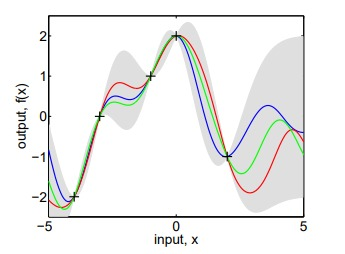
\includegraphics[width = 0.55\textwidth]{graph.jpeg}
    \caption{Graphical Representation}
\end{figure}

Here in this figure you can see that the points marked as \texttt{+} are the points in our dataset, for which the output is exactly one value while it is a distribution (as given by the shaded area) for all the other points

\section{Gaussian Process}

Gaussian processes are a method for non parametric estimation to provide confidence on the seen data and some kind of distribution on unseen data. For any subset of the training data, we must have that the joint prior distribution of this subset is normally distributed for some mean and covariance matrix. For any subset $\{x_1 ... x_m\}$ of the training data, the prior distribution follows:

\[
\begin{bmatrix}
    f(x_1) \\
    \vdots \\
    f(x_m) \\
\end{bmatrix}
\quad \sim \quad
\mathcal{N} (\vec{\mu} (x_1,\dots ,x_m),\Sigma (x_1,\dots,x_m) )
\]
\\
where $\vec{\mu}$ and $\Sigma$ are deterministic functions.


On introducing a new data point into any subset of the training data, we expect the resulting conditional distribution to also follow the normal distribution. For the data point $x^*$

\[
f(x^*) \vert (f(x_1), \dots f(x_m), x^*) \sim \mathcal{N}(\vec{\mu}(x_1,\dots,x_m,x^*), \Sigma(x_1,\dots,x_m,x^*))
\]



As described earlier, we expect that if a new data point introduced is already in the training data, then we expect that $f(x^*)$ takes the value that was present in the training set. This means that for any $x^*$ such that $x^* \in \{x_1,\dots,x_m\} $


\[
f(x^*) \vert (f(x_1), \dots f(x_m), x^*) \sim \mathcal{N}(f(x^*), 0)
\]

Our aim is to design a matrix $\Sigma$ that satisfies such a property i.e. posterior for any point in training data must have zero variance.


 Let $X_{D} = [X^{d}_1 X^{d}_2 \dots X^{d}_n]^T$ denote the points in train set and $X_{T} = [X^{t}_1 X^{t}_2 \dots X^{t}_n]^T$ denote the points in test set. $f(X_D)$ and $f(X_T)$ denote random variables depending on the input.
\[f(X) = 
\begin{pmatrix}
    f(X^{d}_{1})\\
    f(X^{d}_{2})\\
    .\\
    .\\
    f(X^{t}_{n})\\
\end{pmatrix}
\]
These random variables are dependent on each other, and we need to model the dependency between them. We model $f(X)$ as multi-variate Gaussian distribution. Therefore,
\[
\begin{bmatrix}
    f(X_{D}) \\
    f(X_{T}) \\
\end{bmatrix} \sim 
\mathcal{N}
\left(
\begin{bmatrix}
    m(X_{D}) \\
    m(X_{T}) \\
\end{bmatrix}
,
\begin{bmatrix}
    k(X_{D}, X_{D}) &  k(X_{D}, X_{T})\\
    k(X_{D}, X_{T})^{T} & k(X_{T}, X_{T}) \\
\end{bmatrix}
\right)
\]
Here, $m(\cdot)$ is a function denoting mean, and $k(\cdot,\cdot)$ is a kernel function used for creating the covariance matrix. The reason we are using kernel function here is because we want to model some sort of similarity between the random variables, high correlation implying higher similarity. With this model, we can determine the prior distribution of the random variables $f(\cdot)$
\[
P(f(X))=
P
\left(
\begin{bmatrix}
    f(X_{D}) \\
    f(X_{T}) \\
\end{bmatrix}
\right)=
\frac{1}{\text{(some constant)}\cdot \det(K)^{0.5} }
\exp(-0.5f(X)^{T}\Sigma^{-1}f(X))
\]

Our aim now is to get distribution of $f(X_{T})$ given the train predictions $\{y_{i}\}$ and $X_T$. for which we can use Bayes' rule.

\subsection{Evaluating the posterior}
We would model the predictions $Y = [y_{1} y_{2} \dots y_{n}]^{T}$ as 
\[Y = I\cdot f(X_{D})\]
A more general model would be to include additive Gaussian noise  such that $Y = f(X_D) + \eta $. But for simplicity, we assume noise to be zero.
Before the actual derivation, we note two important results.

\subsubsection{Gaussian Marginalisation Rule}
\textbf{If we marginalize out variables in a multivariate Gaussian distribution, the result is still a Gaussian distribution. }Mathematically, if $X=[X_1, X_2, \dots X_n]^{T}$ is a multi-variate Gaussian random variable($\sim \mathcal{N}(\mu, \sigma)$), then any subset of $X$ is a multi-variate Gaussian and the mean and covariance is given by $(A\mu, A\sigma A^{T})$. $A$ can be constructed by using $e_{i}^{T}$ as rows. For example, if $n=3$, and the subset is constructed using $[X_{1}\text{ }X_{3}]$, then,
\[A = 
\begin{pmatrix}
    1 & 0 & 0 \\
    0 & 0 & 1 \\
\end{pmatrix}
\]

\subsubsection{Conditional Rule for multi-variate Gaussian}
Intuitively, if we start with a Gaussian distribution and update our knowledge given the observed value of one of its components(that is, find conditional probability distribution), then the resulting distribution is still Gaussian! Mathematically,\\
Let $[x \text{ }y]$ jointly form multi variate Gaussian random variable,
\[
\begin{bmatrix}
    x \\
    y \\
\end{bmatrix} \sim
\mathcal{N}
\left(
\begin{bmatrix}
    \mu_x \\
    \mu_y \\
\end{bmatrix},
\begin{bmatrix}
    \Sigma_{xx} & \Sigma_{xy}\\
    \Sigma_{yx} & \Sigma_{yy}\\
\end{bmatrix}
\right)
\]

Here $\Sigma_{ab}$ represents covariance matrix between random vectors $a$ and $b$ and $f(\cdot)$ represents the PDF.

\[f(x\vert y) = \frac{f(x,y)}{f(y)}\]
Now, we will substitute $f(x,y)$ with the expression for multi-variate Gaussian distribution($\mathcal{N}(\mu, \Sigma)$), and $f(y)$ with $\mathcal{N}(\mu_{y}, \Sigma_{yy})$. 
Simplifying the equations, we get
\[
f(x\vert y)=
\mathcal{N}
(\Sigma_{xy}\Sigma_{yy}^{-1}y,
\Sigma_{xx} - \Sigma_{xy}\Sigma_{yy}^{-1}\Sigma_{yx})
\]
($\mu$ is assumed to be zero for simplicity)\\
To get the detailed derivation, please see \cite{prop}
\begin{figure}[h] 
    \begin{center}      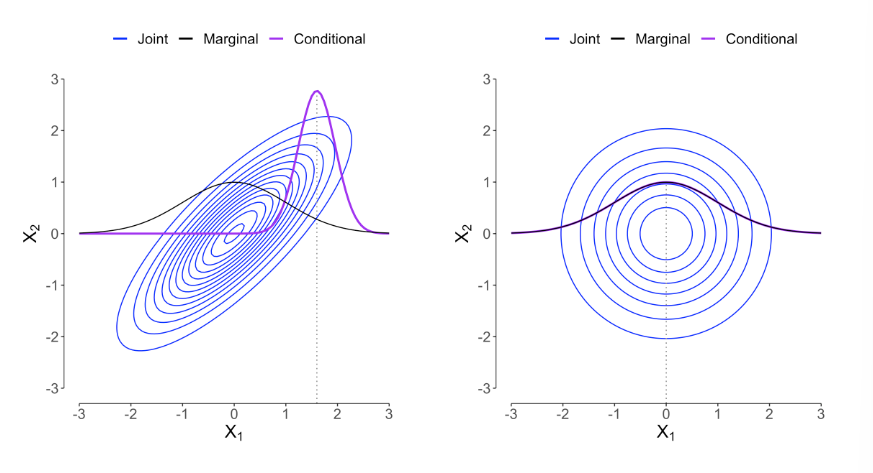
\includegraphics[width=0.8\textwidth]   {rules.png} 
    \caption{Joint, Marginal, Conditional for bivariate Gaussian. Source\cite{prop}}
    \end{center} 
\end{figure}

\subsection{Getting to the posterior}
We modelled $Y=f(X_D)$, now's the time to use it.
\[
\begin{bmatrix}
    f(X_{T}) \\
    Y \\
\end{bmatrix}
\sim 
\mathcal{N}
\left(
\begin{bmatrix}
    \mu(X_{T}) \\
    \mu(X_{D}) \\
\end{bmatrix},
\begin{bmatrix}
    k(X_{T}, X_{T}) &  k(X_{T}, X_{D})\\
    k(X_{T}, X_{D})^{T} &  k(X_{D}, X_{D})\\
\end{bmatrix}
\right)
\]
Using the conditional rule described above,
\[
P(f(X_{D})\vert Y) = \mathcal{N}(\mu_{posterior}, \sigma_{posterior}^2)
\]
where
\[
\mu_{posterior} = \mu{X_{T}} + k(X_{T}, X_{D})(k(X_{D},X_{D}))^{-1}(Y-\mu(X_{D}))\\
\]
\[
\sigma_{posterior}^{2} = k(X_T,X_T) - k(X_T, X_D)(k(X_{D},X_{D}))^{-1}k(X_T, X_D)^{T}
\]



\section{Aftermath\footnote{pun intended (credits Group 31)}}.
\subsection{Posterior mean}
For the sake of investigation, let's assume $\mu(\cdot) = 0$. \\
Now, if $X_{D} = X_{T}$, $\mu_{posterior} = Y$ which is desirable because we want the mean for predictions at training points to be the same as the given predictions in train set. The mean value at a single test location, say $x_{i}^{t}$, is a weighted sum of all the observations Y. The weights are defined by the kernel between the test location $x_{i}^{t}$ and all training locations in X.

\subsection{Posterior variance}
Observe that if $X_{D} = X_{T}$, we get $\sigma_{posterior} = 0$. This means that the prediction for a point in train set is exactly the mean, which in turn is the $Y$ of the training set. 

%\subsection{Example}
%This 
%example is taken from here \cite{blog}.
%The train set is generated by random sampling $x\sim$U([$0, 2\pi$]), and $y=Sin(x) + \eps(noise)$. The blue bands represent a 95\% confidence interval. Notice that for test points near the train points, variance is quite low and ultimate zero at exactly the train points.

%\begin{figure}[h] 
%    \begin{center}      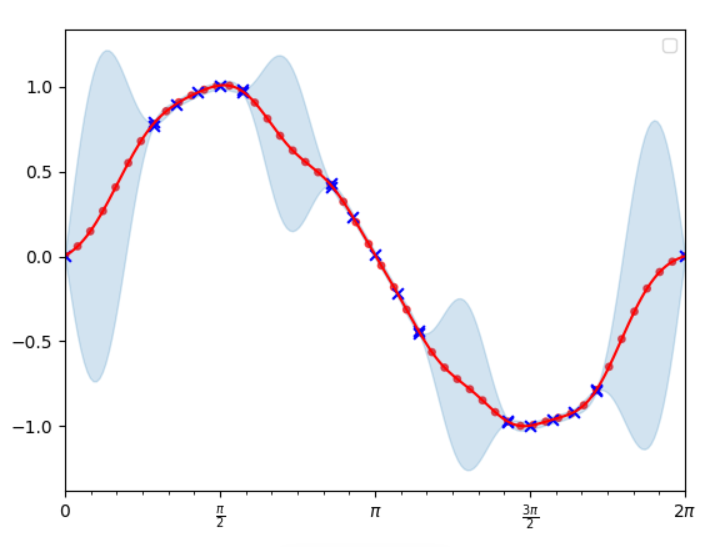
\includegraphics[width=0.6\textwidth]   {sin_eg.png} 
%    \caption{Red points are for test points, and blue ones for train points}
%    \end{center} 
%\end{figure}

\section{Conclusion}
We started with a train set \{($x^{d}_i, y^{d}_i$)\} and test inputs \{$x^{t}_{i}$\}, and devised a function that would yield no error for inputs which are in train set, and low errors on other points. The described method is particularly useful for low data situations. A detailed study of Gaussian processes can be found in the reference \cite{gaussianprocessmachinelearning}.

\clearpage

%%%%%%%%%%% If you don't have citations then comment the lines below:
%
\printbibliography      


%%%%%%%%%%% end of doc
\end{document}